\documentclass[11pt,a4paper]{article}

% CS6868 Research Mini-Project Report
\usepackage[utf8]{inputenc}
\usepackage[T1]{fontenc}
\usepackage[margin=1in]{geometry}
\usepackage{microtype}
\usepackage{lmodern}
\usepackage{amsmath,amssymb}
\usepackage{graphicx}
\usepackage{booktabs}
\usepackage{longtable}
\usepackage{array}
\usepackage{enumitem}
\usepackage{xcolor}
\usepackage{listings}
\usepackage{hyperref}
\usepackage[capitalise,noabbrev]{cleveref}

\graphicspath{{report_figures/}}

\hypersetup{
  colorlinks=true,
  linkcolor=black,
  citecolor=blue!60!black,
  urlcolor=blue!60!black,
}

\definecolor{codegray}{gray}{0.95}
\lstset{
  basicstyle=\ttfamily\small,
  backgroundcolor=\color{codegray},
  frame=single,
  framesep=4pt,
  breaklines=true,
  columns=fullflexible,
  keepspaces=true,
  showstringspaces=false,
}

\title{%
  \textbf{CS6868 Research Mini-Project} \\[0.3em]
  \Large Alloc-free-gc: Allocation-conscious Semi-space Garbage Collection in OxCaml%
}
\author{%
  Aditya Sawant \\ \texttt{CS23B003}
}
\date{\today}

\begin{document}
\maketitle

\begin{abstract}
\texttt{Alloc-free-gc} is an independent experimental garbage-collection
runtime for a small OCaml-style language implementation. The central experiment
is to test whether a garbage collector that avoids heap allocation during
collection can outperform a normal OCaml collector. OxCaml was chosen because it
provides zero-allocation checking and stack-oriented allocation semantics, which
make it possible to write collector hot paths that use stack/local state instead
of allocating ordinary OCaml heap objects. The implementation compares a normal
OCaml semi-space collector against a family of allocation-free variants:
\texttt{zero}, \texttt{zero\_offheap}, \texttt{zero\_offheap\_threaded}, and
\texttt{zero\_stack\_threaded}. On the checked-in benchmark matrix,
\texttt{zero\_offheap} has the best aggregate mean time, 4.914 seconds versus
5.127 seconds for \texttt{normal}. The plots show the expected pattern: the
allocation-free variants often do slightly better, especially at larger
workloads, but their extra FFI, metadata, and worker-thread coordination
overheads sometimes erase the gain. Since each configuration has one run, the
result is directional rather than statistically conclusive.
\end{abstract}

% =============================================================================
\section{Goals}
\label{sec:goals}
% =============================================================================

The goal of this project was to answer a specific performance question: if the
collector itself avoids heap allocation and uses stack/local state during
collection, is it faster than a normal collector written in ordinary OCaml? This
question motivated the choice of OxCaml. OxCaml supports zero-allocation checks
and stack-oriented programming features, so it is a natural tool for building a
collector whose hot path does not allocate into the OCaml heap while the
collector is already trying to recover memory.

The collector algorithm is a stop-the-world semi-space copying collector. This
algorithm is simple enough to implement completely, but still exercises the
runtime-system mechanisms that matter for the experiment: explicit root
discovery, object copying, forwarding pointers, heap-space swapping, and
multi-threaded mutator coordination.

The project connects to CS6868 topics in two ways. First, the runtime uses
threads, shared state, condition variables, and stop-the-world synchronization,
which are direct applications of concurrent programming and synchronization
ideas. Second, several variants change how the runtime crosses the boundary
between C and OCaml/OxCaml, which makes the project a practical study of
contention, coordination overhead, and implementation tradeoffs in systems with
multiple execution contexts.

The research question is:

\begin{quote}
Does a semi-space collector written using OxCaml's zero-allocation and
stack-oriented features run faster than a normal OCaml collector when both share
the same C heap and allocation fast path?
\end{quote}

The secondary question is why the answer is not uniform: when the
allocation-free collector is faster, is the gain large enough to overcome the
extra overheads introduced by FFI calls, off-heap metadata access, and
persistent worker-thread coordination?

% =============================================================================
\section{Background}
\label{sec:background}
% =============================================================================

\subsection{Semi-space Copying Collection}

The collector uses the classic semi-space copying strategy. The heap is divided
into two equal regions: from-space and to-space. Mutators allocate linearly in
from-space using a bump pointer. When allocation fails, mutators stop and the
collector copies all reachable objects into to-space. After collection,
from-space and to-space are swapped, and allocation resumes after the copied
live data.

The traversal is Cheney-style breadth-first copying~\cite{cheney1970}. The
collector maintains a \texttt{free\_ptr}, where the next copied object will be
placed, and a \texttt{scan\_ptr}, which walks through objects already copied to
to-space. Roots are copied first. Then the collector scans copied objects and
copies any reachable pointer fields that still point into the old from-space.

\begin{lstlisting}[language=C,caption={High-level semi-space collection sketch.},label={lst:cheney}]
free_ptr = to_space_start;
scan_ptr = to_space_start;

for root in roots:
  root = copy(root, &free_ptr);

while scan_ptr < free_ptr:
  obj = scan_ptr;
  for field in obj.pointer_fields:
    field = copy(field, &free_ptr);
  scan_ptr += object_size(obj);

swap(from_space, to_space);
current_heap_ptr = free_ptr - new_from_space;
\end{lstlisting}

\subsection{Runtime Representation}

The runtime uses an OCaml-style tagged-word representation. Integers have low
bit \(1\), while heap pointers have low bit \(0\). Heap pointers exposed to
program code point to the object body. The object header is stored one word
before the body and records the object size and tag.

During copying, the old object is converted into a forwarding object: the header
is overwritten with a forwarding marker, and the first payload slot stores the
new body pointer. Later visits to the same object can then return the forwarded
address without copying the object again.

\subsection{Root Tracking and Stop-the-world Collection}

Root tracking is explicit. Each mutator has a thread-local stack of root
addresses, a stack index, a return-value root slot, and an active/inactive flag.
The collector scans root addresses and updates them in place after moving
objects.

Collection is stop-the-world. When the allocation path cannot satisfy a request,
the requesting mutator marks a GC request and waits until all active mutators
reach a polling or allocation point. The selected collector variant then runs
with no concurrent mutation.

\subsection{Why OxCaml and Stack-oriented Allocation}

A collector is a particularly sensitive place to allocate ordinary heap objects:
it runs exactly when the runtime has failed to satisfy an allocation request.
If the collector implementation itself allocates on the managed heap, then its
bookkeeping can perturb the measurement and may introduce additional runtime
pressure. The purpose of using OxCaml was therefore not merely to reimplement a
collector in another language; it was to use OxCaml's zero-allocation checking
and stack-oriented semantics to keep the collector hot path allocation-free.

The ideal target is a collector whose temporary bookkeeping lives in bounded
locals or stack-backed state, while persistent metadata either remains outside
the OCaml heap or is accessed without allocating. The variants in this project
are successive approximations of that target.

% =============================================================================
\section{Tasks Undertaken}
\label{sec:tasks}
% =============================================================================

\subsection{Implementation}

The project is organized into three layers.

\begin{itemize}[leftmargin=*]
  \item \textbf{Runtime layer}: \texttt{runtime.c} and \texttt{runtime.h}
  define tagged-value helpers, allocation entry points, mutator thread startup,
  explicit root registration, and stop-the-world coordination.
  \item \textbf{FFI and heap layer}: \texttt{gc\_ffi.c} embeds the OCaml/OxCaml
  runtime, owns the semi-space heap, exposes the \texttt{mmtk\_*} ABI consumed
  by the runtime layer, and provides no-allocation C stubs for raw memory
  access.
  \item \textbf{Collector layer}: one OCaml/OxCaml module is selected at build
  time through the Makefile variable \texttt{GC=}.
\end{itemize}

The implemented collector variants are:

\paragraph{Normal OCaml collector.}
\texttt{gc\_normal.ml} is the baseline. It implements the same semi-space
algorithm using ordinary OCaml references and arrays for metadata. This gives a
direct comparison point for the allocation-free hypothesis: if ordinary OCaml
allocation in collector bookkeeping is not a significant cost, this baseline
should be hard to beat.

\paragraph{Zero-allocation OxCaml collector.}
\texttt{gc.ml}, selected by \texttt{GC=zero}, rewrites the hot collection path
with OxCaml zero-allocation annotations. The copy function returns both the
updated pointer and next free pointer without allocating an OCaml pair. This is
the first direct test of the main idea: make the collector's active copying and
scanning path allocation-free.

\paragraph{Off-heap metadata collector.}
\texttt{gc\_zero\_offheap.ml}, selected by \texttt{GC=zero\_offheap}, moves
persistent metadata into malloc-backed memory. Static root slots, mutator root
stack pointers, stack-index pointers, return-root pointers, active-thread flags,
and counters are accessed through no-allocation C stubs. This was added because
the plain \texttt{zero} collector still keeps long-lived metadata in OCaml
arrays; moving that state off-heap makes the implementation closer to the
intended allocation-free collector model.

\paragraph{Threaded off-heap collector.}
\texttt{GC=zero\_offheap\_threaded} uses the same off-heap collector but runs
collection through a persistent sleeping GC worker thread. Allocation failure
wakes the worker after mutators have stopped.

\paragraph{Stack-threaded collector service.}
\texttt{gc\_stack\_threaded.ml}, selected by
\texttt{GC=zero\_stack\_threaded}, runs collection inside a long-lived OxCaml
service loop. C owns mutator metadata; the OxCaml service thread performs only
collection when it receives a command. This variant most directly targets the
``use stack space for GC work'' idea: the collector logic runs in a persistent
worker frame, so stack-local state can remain within a long-lived collection
service rather than being recreated through normal callback paths.

\subsection{Testing and Verification}

Correctness was tested at three levels.

\begin{itemize}[leftmargin=*]
  \item \textbf{Smoke test}: \texttt{smoke\_test.c} allocates small linked
  objects, writes fields, and reads them back through the runtime API.
  \item \textbf{Single-threaded tree benchmark}: \texttt{benchmarks/binary\_tree.c}
  builds stretch, temporary, and long-lived trees and checks node-count
  traversals after allocation and collection.
  \item \textbf{Multi-threaded tree benchmark}:
  \texttt{benchmarks/binary\_tree\_multithreaded.c} runs the same allocation
  pattern across multiple worker threads and checks that all workers complete
  with the expected tree checksums.
\end{itemize}

The benchmark is not a formal proof of collector correctness, but it exercises
the important invariants for this project: roots must be updated after copying,
return values must survive allocation during nested calls, long-lived objects
must remain reachable, and stopped mutators must resume with valid pointers.

% =============================================================================
\section{Evaluation}
\label{sec:evaluation}
% =============================================================================

\subsection{Experimental Setup}

The main benchmark driver is
\texttt{benchmarking/run\_gc\_benchmark.sh}. It rebuilds
\texttt{binary\_tree\_multithreaded\_test} once per collector variant and records
elapsed wall-clock time. The checked-in result matrix uses:

\begin{itemize}[leftmargin=*]
  \item depths 11, 12, 13, and 14;
  \item mutator thread counts 1 through 8;
  \item variants \texttt{normal}, \texttt{zero}, \texttt{zero\_offheap},
  \texttt{zero\_offheap\_threaded}, and \texttt{zero\_stack\_threaded};
  \item one run per configuration.
\end{itemize}

The plotting script \texttt{benchmarking/plot\_gc\_benchmark.py} produces
per-depth time plots, summary statistics, and normal-relative speedup ratios.
Since the checked-in data have one run per configuration, the evaluation should
be read as directional. Repeated measurements are required for strong
quantitative claims.

\subsection{Pilot Benchmark: Does Zero-allocation Help?}

An older pilot run compared only the normal OCaml and zero-allocation OxCaml
collectors. It is included because it was the first measurement of whether
zero-allocation annotations helped end-to-end runtime.

\begin{figure}[h]
  \centering
  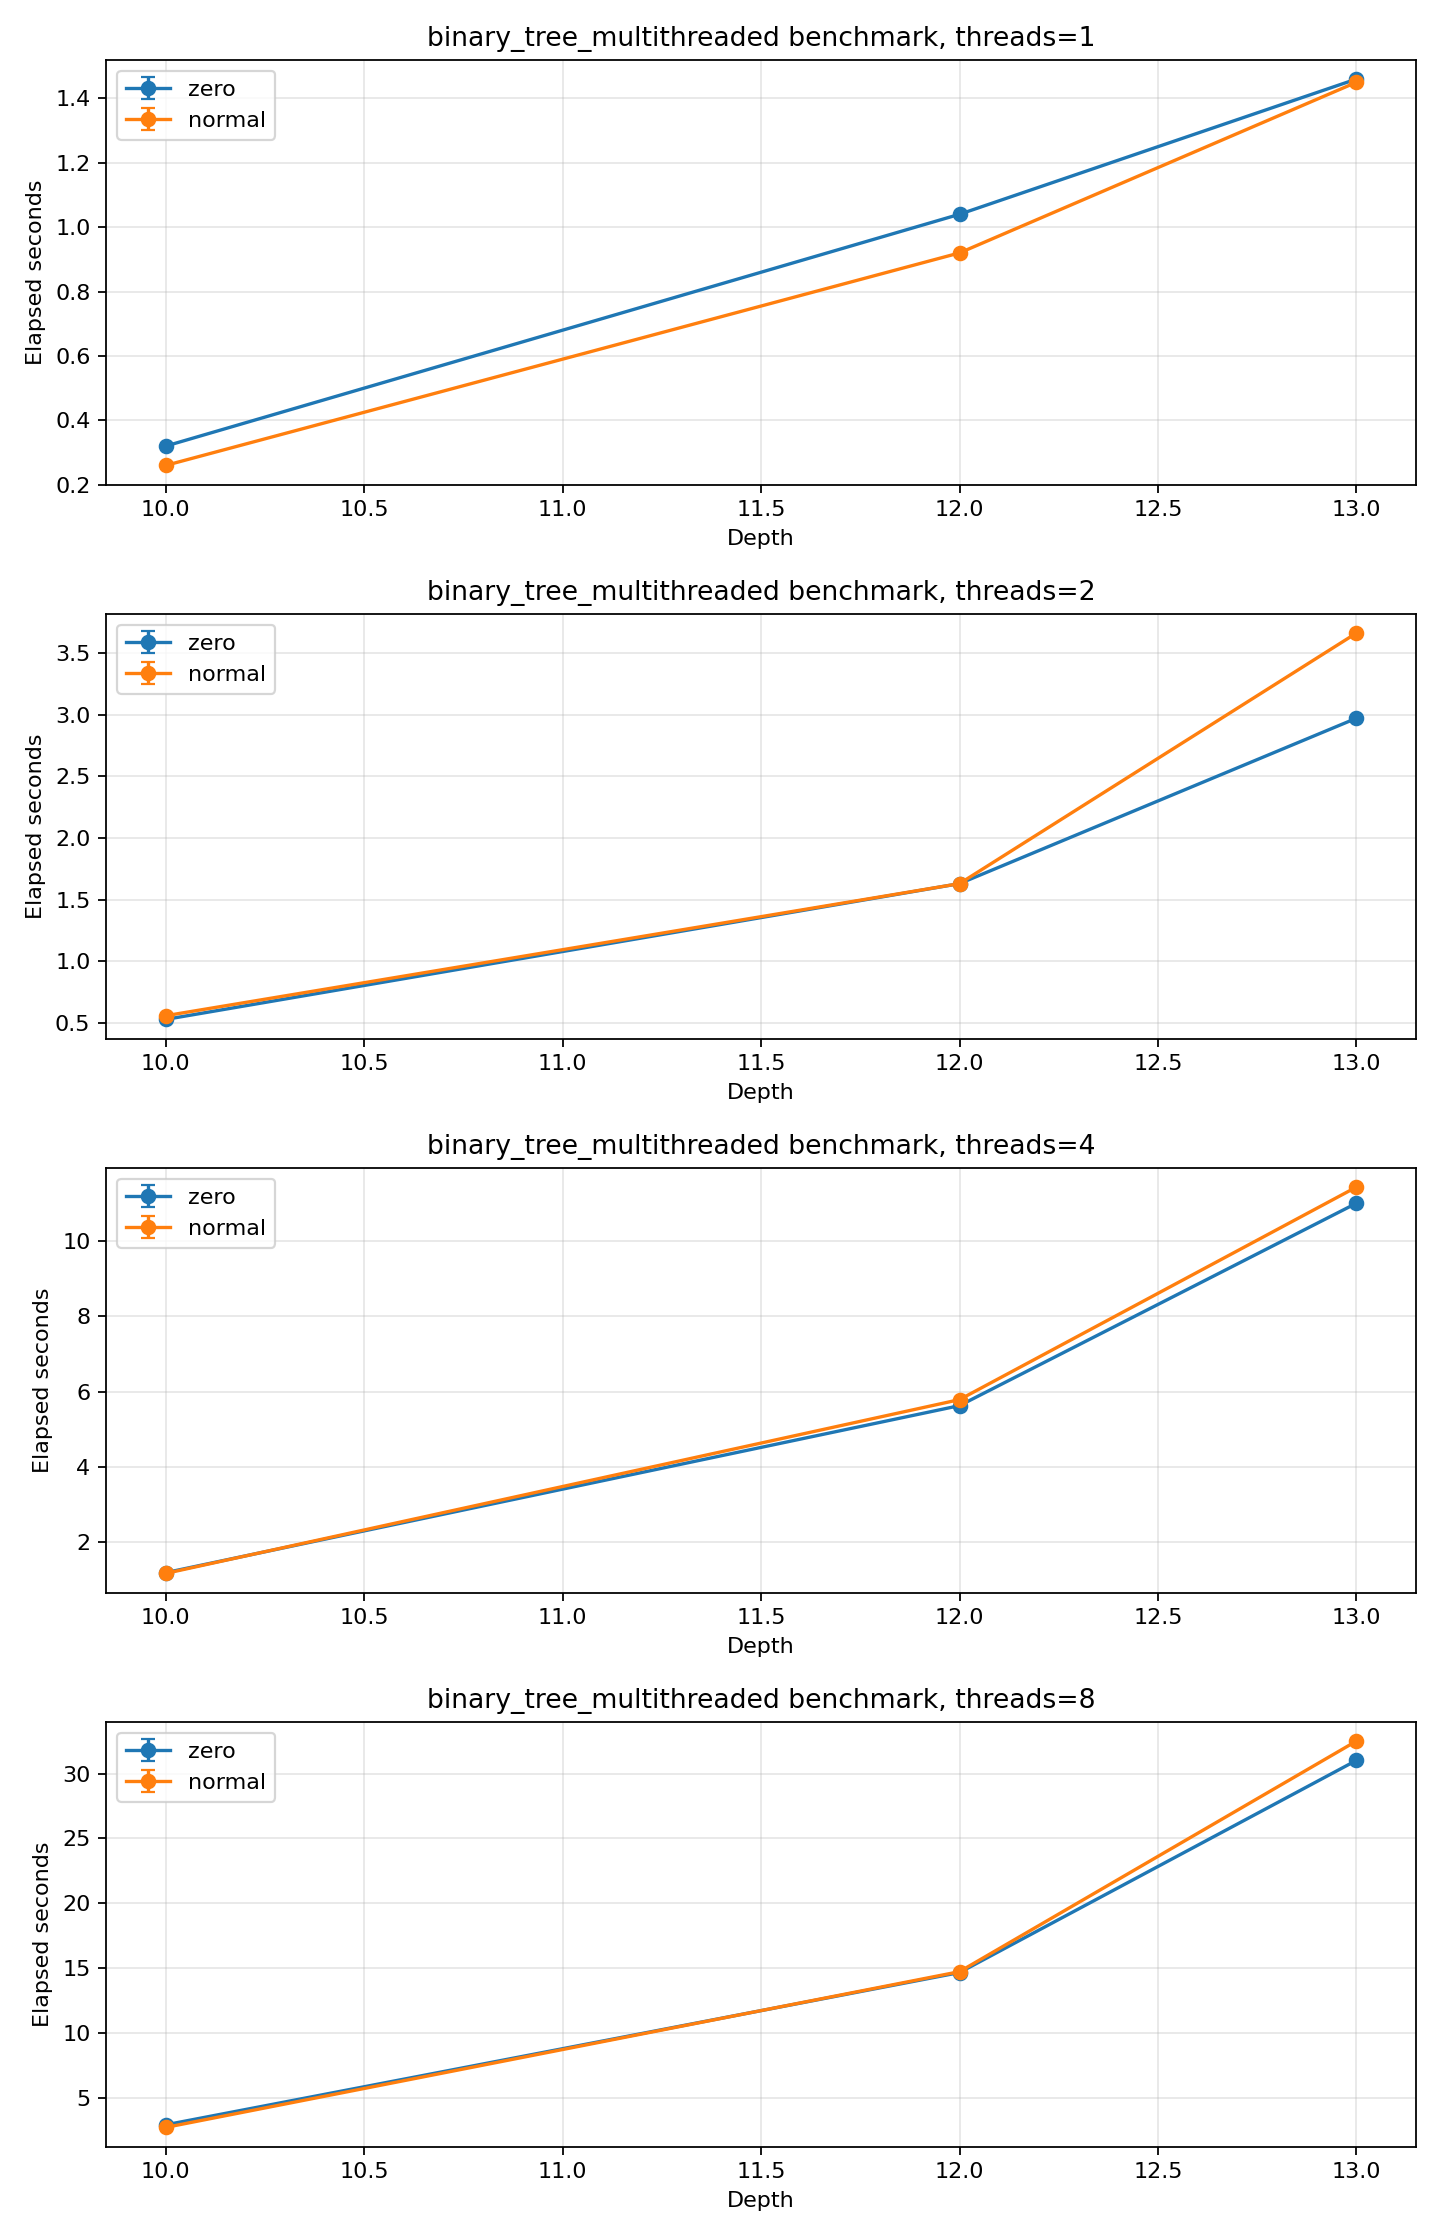
\includegraphics[width=0.75\linewidth]{pilot_normal_vs_zero.png}
  \caption{Pilot benchmark comparing the normal OCaml collector and the
  zero-allocation OxCaml collector.}
  \label{fig:pilot}
\end{figure}

\begin{table}[h]
\centering
\caption{Pilot benchmark summary. Ratio is normal/zero, so values above 1.0
favor the zero-allocation collector.}
\label{tab:pilot}
\begin{tabular}{rrrrr}
\toprule
Depth & Threads & Normal & Zero & Ratio \\
\midrule
10 & 1 & 0.26 & 0.32 & 0.812 \\
10 & 2 & 0.56 & 0.53 & 1.057 \\
10 & 4 & 1.17 & 1.19 & 0.983 \\
10 & 8 & 2.72 & 2.92 & 0.932 \\
12 & 4 & 5.79 & 5.63 & 1.028 \\
13 & 2 & 3.66 & 2.97 & 1.232 \\
13 & 8 & 32.51 & 31.02 & 1.048 \\
\bottomrule
\end{tabular}
\end{table}

The pilot mean over its 12 configurations was 6.403 seconds for
\texttt{normal} and 6.198 seconds for \texttt{zero}. This supports the initial
hypothesis only weakly. The allocation-free collector is not automatically
faster at small depths: for example, at depth 10 with 1 and 8 threads it is
slower than \texttt{normal}. But at larger depth/thread combinations, such as
depth 13 with 2, 4, and 8 threads, \texttt{zero} is faster. This suggests that
removing collector-side heap allocation can help when the workload is large
enough, but the benefit must first overcome fixed overheads from callback
crossing, root metadata access, and raw memory operations.

\subsection{Main Benchmark Results: Allocation-free Family vs. Normal GC}

\begin{table}[h]
\centering
\caption{Aggregate timing over 32 configurations per variant. Mean is the
arithmetic mean of per-configuration elapsed time.}
\label{tab:aggregate}
\begin{tabular}{lrrrr}
\toprule
Variant & Mean (s) & Min (s) & Max (s) & Faster than normal \\
\midrule
\texttt{normal} & 5.127 & 0.25 & 28.69 & baseline \\
\texttt{zero} & 5.038 & 0.26 & 26.79 & 16 / 32 \\
\texttt{zero\_offheap} & 4.914 & 0.21 & 26.68 & 21 / 32 \\
\texttt{zero\_offheap\_threaded} & 4.919 & 0.23 & 26.11 & 17 / 32 \\
\texttt{zero\_stack\_threaded} & 5.013 & 0.24 & 30.42 & 20 / 32 \\
\bottomrule
\end{tabular}
\end{table}

The aggregate result answers the main question cautiously. Every
allocation-free variant except the plain \texttt{zero} variant's consistency
problem is competitive with \texttt{normal}, and the best mean is from
\texttt{zero\_offheap}. The improvement from 5.127 seconds to 4.914 seconds is
about 4.2 percent. That is meaningful enough to suggest that avoiding
collector-side heap allocation can pay off, but not large enough to claim that
stack/zero-allocation semantics dominate all other costs.

\begin{figure}[h]
  \centering
  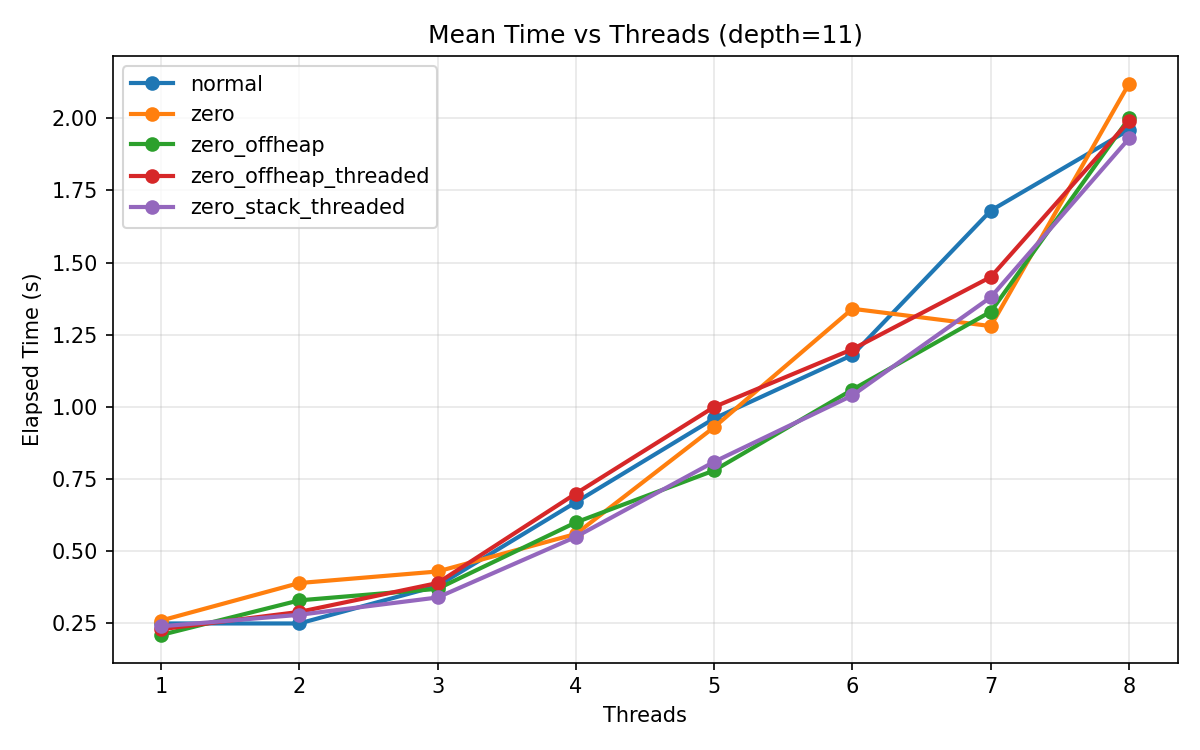
\includegraphics[width=0.48\linewidth]{time_vs_threads_depth_11.png}
  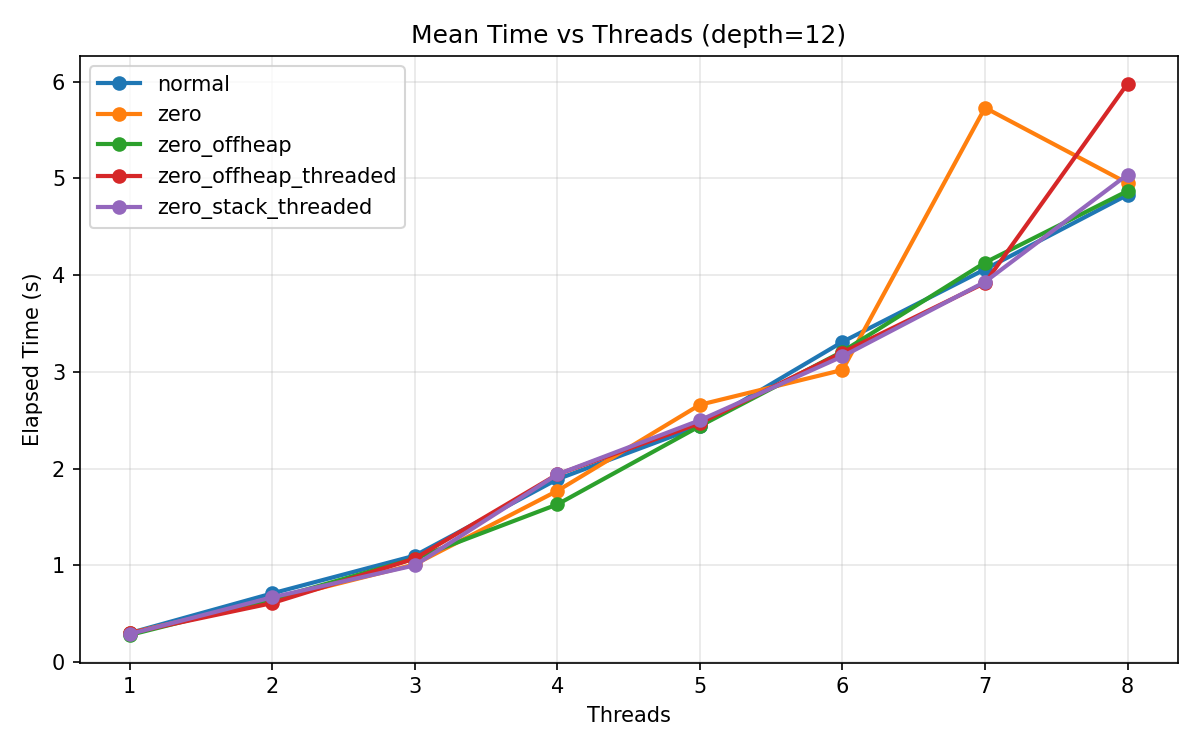
\includegraphics[width=0.48\linewidth]{time_vs_threads_depth_12.png}
  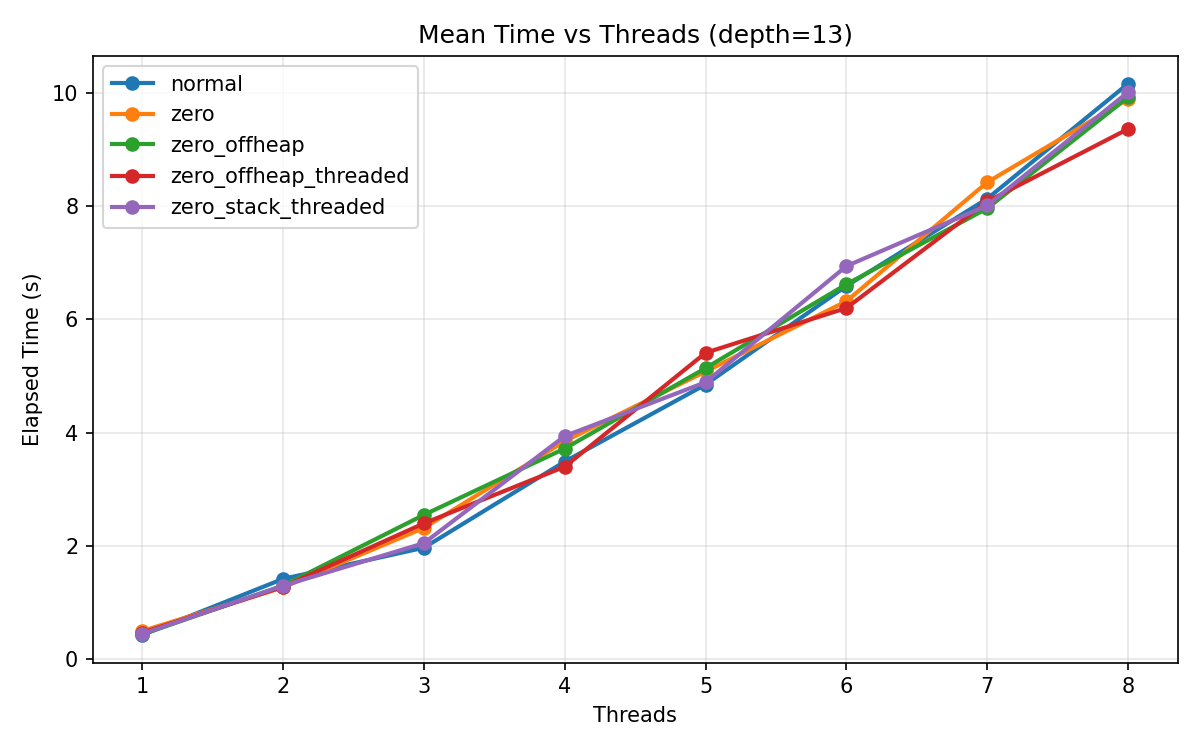
\includegraphics[width=0.48\linewidth]{time_vs_threads_depth_13.png}
  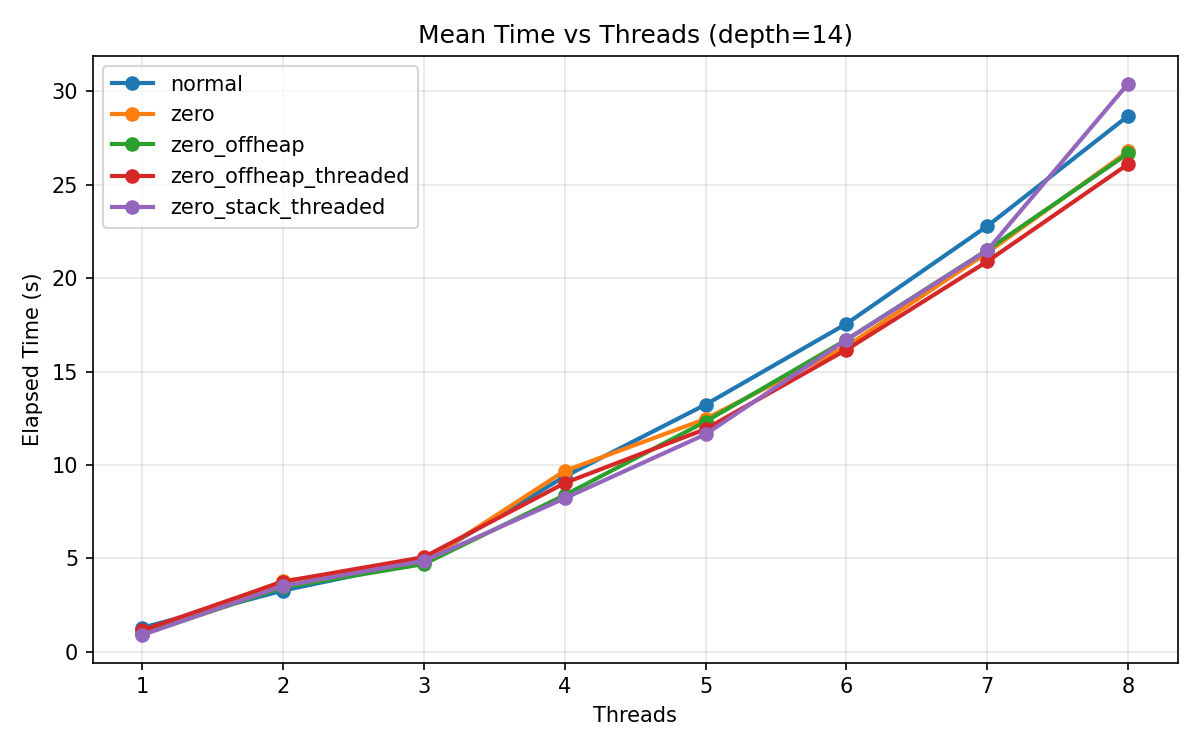
\includegraphics[width=0.48\linewidth]{time_vs_threads_depth_14.png}
  \caption{Elapsed time versus mutator threads for depths 11--14.}
  \label{fig:time-curves}
\end{figure}

\begin{figure}[h]
  \centering
  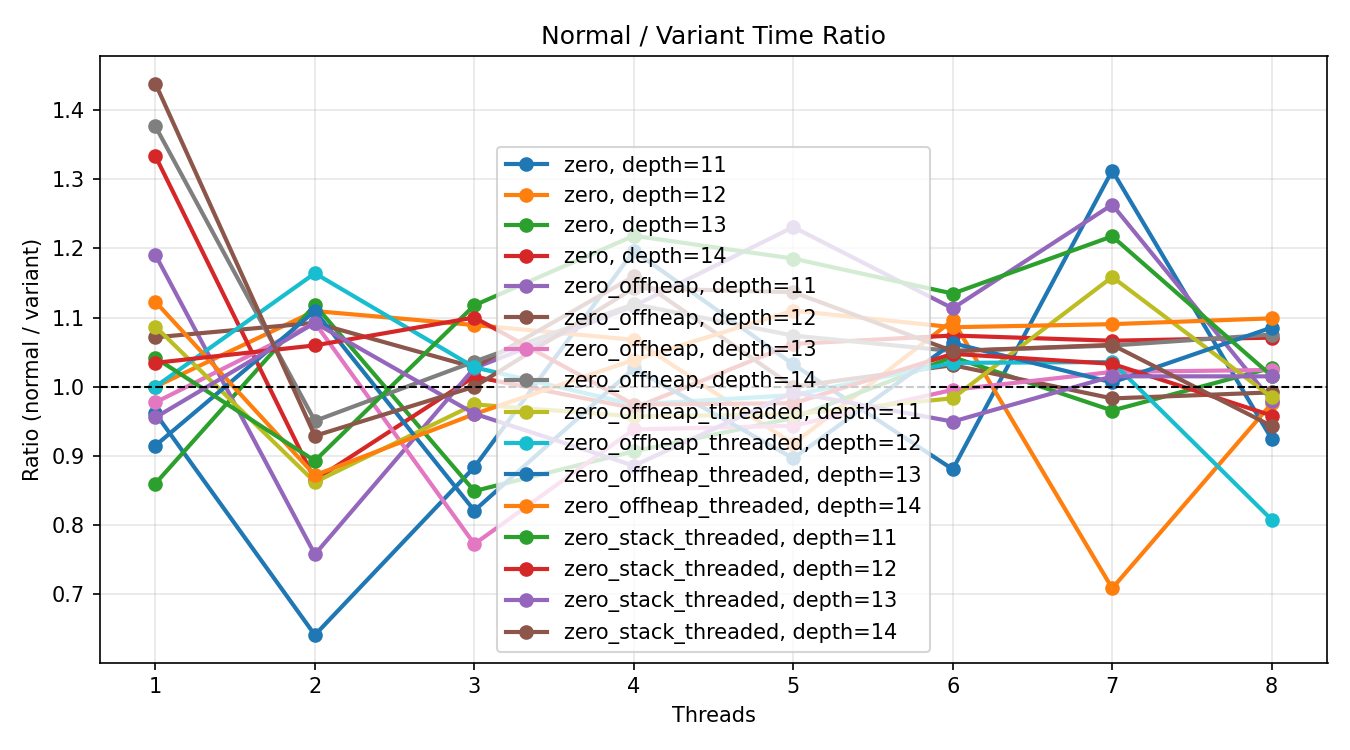
\includegraphics[width=0.88\linewidth]{normal_relative_speedup.png}
  \caption{Normal/variant time ratios. Values above 1.0 mean the variant is
  faster than the normal OCaml baseline.}
  \label{fig:speedup}
\end{figure}

\subsection{Discussion and Inferences from the Plots}

The plots show that the original hypothesis is partly true. The
allocation-free family often sits slightly below the normal collector, but the
lines are close and cross several times. That shape is important: it means the
experiment did not uncover a large algorithmic speedup, but it did show that
collector-side heap allocation is one contributor to total runtime.

\paragraph{Zero-allocation alone helps only when the workload is large enough.}
The plain \texttt{zero} variant is faster in exactly half of the measured
configurations. At smaller depths, the cost saved by avoiding heap allocation in
the collector is comparable to or smaller than the overhead of the OxCaml/C
callback path and no-allocation memory stubs. At larger configurations, such as
several depth-14 cases, \texttt{zero} becomes faster than \texttt{normal}. This
matches the expected threshold behavior: fixed overheads dominate small runs,
while allocation-free collection has more opportunity to pay off in larger
runs.

\paragraph{Off-heap metadata is the clearest improvement.}
The most promising variant is \texttt{zero\_offheap}. It is faster than normal
in 21 of 32 configurations and has the lowest aggregate mean. This supports a
more precise version of the hypothesis: it is not enough for the copy loop to be
zero-allocation if persistent root and thread metadata still live in OCaml
arrays. Moving metadata out of the OCaml heap makes the collector closer to the
intended model, where GC bookkeeping does not allocate or depend on managed heap
state.

\paragraph{The stack-threaded design exposes the cost of making stack state
long-lived.}
\texttt{zero\_stack\_threaded} was intended to make stack-local collector state
practical by running collection inside a persistent service loop. It performs
well in several configurations: at depth 14 with 1, 4, and 5 threads it is the
fastest variant. However, it is also the slowest at depth 14 with 8 threads
(30.42 seconds versus 28.69 for \texttt{normal}). This is the clearest example
of overheads adding up. The service-thread command queue and synchronization
can erase the benefit of stack-local state when mutator coordination pressure is
high.

\paragraph{Threaded off-heap is useful at larger high-thread cases.}
\texttt{zero\_offheap\_threaded} is strongest near the larger end of the matrix:
it is the fastest variant at depth 13 with 4, 6, and 8 threads, and at depth 14
with 6, 7, and 8 threads. This suggests that a persistent worker can help when
the collection workload is large enough to amortize the worker coordination
cost. It also explains why the threaded variant is not consistently best at
smaller depths.

\paragraph{Overall inference.}
The meaningful result is therefore not ``allocation-free GC is always faster.''
The more accurate conclusion is: an allocation-free collector built using
OxCaml's zero-allocation/stack-oriented features can be slightly faster than a
normal OCaml collector, but only when the saved heap-allocation overhead exceeds
the extra overhead introduced by FFI boundaries, off-heap metadata access, and
thread/service coordination.

\begin{longtable}{rrrrrrr}
\caption{Main benchmark elapsed time by configuration. Times are seconds.}
\label{tab:detail}\\
\toprule
Depth & Threads & Normal & Zero & Offheap & Offheap-thr & Stack-thr \\
\midrule
\endfirsthead
\toprule
Depth & Threads & Normal & Zero & Offheap & Offheap-thr & Stack-thr \\
\midrule
\endhead
11 & 1 & 0.25 & 0.26 & 0.21 & 0.23 & 0.24 \\
11 & 2 & 0.25 & 0.39 & 0.33 & 0.29 & 0.28 \\
11 & 3 & 0.38 & 0.43 & 0.37 & 0.39 & 0.34 \\
11 & 4 & 0.67 & 0.56 & 0.60 & 0.70 & 0.55 \\
11 & 5 & 0.96 & 0.93 & 0.78 & 1.00 & 0.81 \\
11 & 6 & 1.18 & 1.34 & 1.06 & 1.20 & 1.04 \\
11 & 7 & 1.68 & 1.28 & 1.33 & 1.45 & 1.38 \\
11 & 8 & 1.96 & 2.12 & 2.00 & 1.99 & 1.93 \\
12 & 1 & 0.30 & 0.30 & 0.28 & 0.30 & 0.29 \\
12 & 2 & 0.71 & 0.64 & 0.65 & 0.61 & 0.67 \\
12 & 3 & 1.10 & 1.01 & 1.07 & 1.07 & 1.00 \\
12 & 4 & 1.89 & 1.77 & 1.63 & 1.94 & 1.94 \\
12 & 5 & 2.44 & 2.66 & 2.44 & 2.47 & 2.50 \\
12 & 6 & 3.31 & 3.02 & 3.21 & 3.20 & 3.16 \\
12 & 7 & 4.06 & 5.73 & 4.13 & 3.92 & 3.93 \\
12 & 8 & 4.83 & 4.95 & 4.87 & 5.98 & 5.04 \\
13 & 1 & 0.43 & 0.50 & 0.44 & 0.47 & 0.45 \\
13 & 2 & 1.42 & 1.27 & 1.30 & 1.28 & 1.30 \\
13 & 3 & 1.97 & 2.32 & 2.55 & 2.40 & 2.05 \\
13 & 4 & 3.49 & 3.85 & 3.72 & 3.40 & 3.94 \\
13 & 5 & 4.85 & 5.08 & 5.14 & 5.41 & 4.89 \\
13 & 6 & 6.59 & 6.32 & 6.62 & 6.20 & 6.94 \\
13 & 7 & 8.13 & 8.42 & 7.96 & 8.08 & 8.01 \\
13 & 8 & 10.16 & 9.89 & 9.92 & 9.36 & 10.01 \\
14 & 1 & 1.28 & 0.96 & 0.93 & 1.14 & 0.89 \\
14 & 2 & 3.27 & 3.78 & 3.44 & 3.75 & 3.52 \\
14 & 3 & 4.86 & 4.79 & 4.69 & 5.06 & 4.86 \\
14 & 4 & 9.38 & 9.68 & 8.38 & 9.03 & 8.21 \\
14 & 5 & 13.23 & 12.46 & 12.32 & 11.92 & 11.64 \\
14 & 6 & 17.56 & 16.35 & 16.70 & 16.17 & 16.70 \\
14 & 7 & 22.79 & 21.37 & 21.51 & 20.90 & 21.49 \\
14 & 8 & 28.69 & 26.79 & 26.68 & 26.11 & 30.42 \\
\bottomrule
\end{longtable}

% =============================================================================
\section{Reflection on the Use of LLMs}
\label{sec:llm}
% =============================================================================

\paragraph{Tools and models used.}
I used ChatGPT/Codex during the project for code navigation, implementation
planning, debugging, benchmark-script cleanup, plotting-script review, and
report drafting. The LLM was also used to reorganize the project into a more
standalone shape and to convert benchmark results into tables and prose.

\paragraph{What worked well.}
The most useful assistance was mechanical but time-saving: comparing collector
variants, summarizing benchmark CSVs, identifying which files were build
artifacts, and generating LaTeX tables from result files. The LLM also helped
reframe the evaluation around the actual hypothesis: whether OxCaml's
zero-allocation and stack-oriented features reduce collector overhead compared
with a normal OCaml implementation.

\paragraph{What did not work.}
The LLM was not reliable as a source of final truth for low-level runtime
behavior. Some early descriptions over-emphasized reference implementations and
later drafts described the project as a collection of variants rather than as a
focused test of allocation-free GC. This was caught by reviewing whether the
report explained why OxCaml was used in the first place.

\paragraph{What was surprising.}
It was useful for quickly turning raw benchmark data into an interpretable
story, but small wording choices mattered a lot. A report can become misleading
if it describes the project as a loose set of attempted variants rather than as
a focused experiment with a clear hypothesis, benchmarks, and results.

\paragraph{What was difficult.}
The LLM could not replace understanding of the collector invariants. Decisions
about root updates, forwarding, stop-the-world coordination, and whether
zero-allocation annotations were actually meaningful had to be checked against
the code and benchmark behavior. In particular, interpreting why an
allocation-free variant can be slower required understanding the overheads of
FFI calls, off-heap metadata access, and persistent service-thread
synchronization.

\paragraph{Your overall assessment.}
The LLM was helpful for acceleration, documentation, and sanity checks, but the
runtime design and performance interpretation still required manual validation.
I would use it again, but only with code review and benchmark verification.

% =============================================================================
\section{Conclusions}
\label{sec:conclusions}
% =============================================================================

The research question was whether a collector written to avoid heap allocation,
using OxCaml's zero-allocation and stack-oriented features, can outperform a
normal OCaml collector behind a shared C allocation fast path. The answer from
the current evidence is: slightly, but not universally. The
\texttt{zero\_offheap} variant has the best aggregate mean and beats the normal
baseline in most configurations, while \texttt{zero\_stack\_threaded} shows
that making stack-local collector state practical can also introduce
synchronization overhead.

The main lesson is that allocation-free GC is a useful optimization direction,
not a free win. It reduces one source of overhead, but total runtime also
depends on root scanning, raw memory access through stubs, copied object volume,
and mutator/worker coordination. The plots are consistent with this: the
allocation-free variants often do better, but the advantage is small and
occasionally reversed.

The main limitation is measurement confidence. The next step is to rerun the
full matrix with 5--10 repetitions per configuration and to separately record
collection count, copied bytes, and GC pause time. That would make it possible
to distinguish collector improvement from mutator scheduling noise and general
runtime overhead.

% =============================================================================
\section*{Contributions}
\label{sec:contributions}
% =============================================================================

\begin{center}
\begin{tabular}{@{}lcl@{}}
\toprule
\textbf{Member} & \textbf{Contribution (\%)} & \textbf{Main responsibilities} \\
\midrule
Aditya Sawant & 100\% & Runtime integration, collector variants, benchmarking, plots, report \\
\midrule
\textbf{Total} & \textbf{100\%} & \\
\bottomrule
\end{tabular}
\end{center}

% =============================================================================
\bibliographystyle{plainurl}
\bibliography{references}
% =============================================================================

\end{document}
